\section{トリガーロジック開発の流れ}
\label{sec_TriggerTestSystem}
図\ref{Trigger_flow}にトリガーロジックの開発フローを示す。トリガーロジックの開発は、概念設計、モジュールごとのHDL実装、全体ファームウェアの統合という3ステップで進められる。
以下でそれぞれのステップについて説明する。

\begin{figure} 
\centering
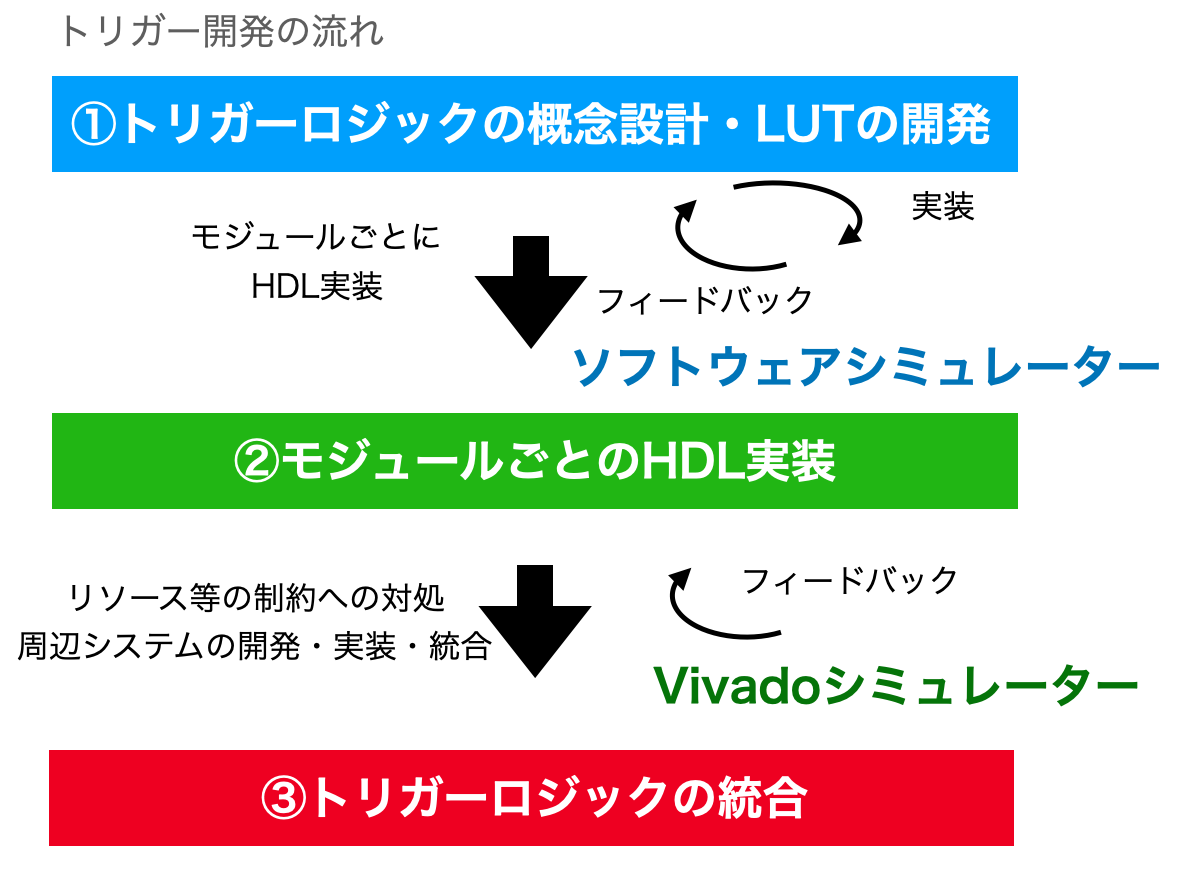
\includegraphics[width=16cm]{fig/SL/Trigger_flow.png}
\caption[TGCトリガー開発の流れ]{トリガーロジック開発の流れ。トリガー開発はまず、検出器からのヒットデータを用いてどのようにコインシデンスロジックを組むか、など概念設計が行われる。次に、その設計をHDLとして実装し、デジタル回路の論理演算へと翻訳する。最後に実装されたトリガーモジュールを全体ファームウェアの中に統合し、システム全体として動作するようになる。概念設計の際にはソフトウェアシミュレーターが、HDL実装の際にはVivado シミュレーターが検証用に用いられる。}
\label{Trigger_flow}
\end{figure}

\subsection*{トリガーロジックの概念設計}
トリガーロジック開発の最初のステップは概念設計である。高輝度LHC-ATLAS実験ではL0 Trigger Systemが従来のものからアップグレードされ、トリガーレートは10倍に、トリガーレイテンシーは4倍に増強される。それに伴い、TGCエレクトロニクスシステムも刷新され、SL FPGAはヒットの有無に関わらず、TGC BWの全7層からのヒットビットマップをすべて受信するようになる。

概念設計の段階では、新しい入力データを利用して、どのようなロジックを構築すれば、L0トリガーシステムの要求 ( 具体的にはトリガー効率、再構成されたミューオンの\pt 分解能、トリガーレート、トリガーレイテンシーなど ) を満たすとともに、より高精度のトリガーを実現できるかを考案する。このプロセスで、ロジックの全体的な設計 (例えば、M1、M2、M3のヒット情報からミューオンの飛跡と無限運動量飛跡がなす角度を算出し、それを利用して \pt を概算する、など) から、具体的な仕様(例えば、複数の飛跡候補がある場合にどの基準で候補を絞り込むか)まで決定する。

設計したロジックを、より具体的なデザインに落とし込む際にはソフトウェアシミュレーターが重要な役割を果たす。ソフトウェアは開発が容易であり、ロジックの実装→性能評価→修正→…という開発サイクルを迅速に進めることが可能である。そのため、グローバルなデザインを決めていく初期の開発では特に有効である。また、パターンマッチングに利用するLUTもロジックの設計と同時に開発される。

\subsection*{モジュールごとのHDL実装}
トリガー開発の次のステップは各モジュールのHardware Description Language ( HDL ) 実装である。この段階では、概念設計で策定したロジックをHDLを通じて、デジタル回路の論理演算へと翻訳する。この工程では、限られたハードウェアリソースの中で、どのように性能を維持したままロジックを実現するか、という物理制約を意識したロジック最適化が重要となる。例えば、パターンマッチングを行うための最小領域の設計などが行われた。パターンマッチングでは多くのチャンネルを入力とした方が、より多くの飛跡パターンをカバーすることができるため、トリガー効率は高くなる。一方、FPGA内で使用できるRAMリソースは限られているため、使用するLUTのサイズには物理的な制限がかかる。トリガー効率を維持したまま、1枚のFPGAでロジックを実現できるよう、最小領域の取り決めが行われた。

実装されたHDLの動作検証および実装されたトリガー回路の性能評価には、Vivado シミュレーターが用いられる。Vivado シミュレーターとはHDLで記述されたデジタル回路の動作を逐次的にエミュレートするソフトウェアツールである。デジタル回路に含まれる全ての信号の遷移を厳密にシミュレーションし、任意の時間の任意の信号線をプローブすることができる。

\subsection*{トリガーロジックの統合}
トリガー開発の最後のステップはトリガーロジックの統合である。この段階では、開発したトリガーモジュールをSLの全体ファームウェアへと適切に組み込む。

統合作業では、トリガー回路をI/O、コントロール回路、読み出し回路と接続する。I/Oは、PS boardや磁場内部からの検出器からのヒット信号を受信するパートで、受信したデータをトリガー入力に適した形に整形し、適切なタイミングでロジックへと投入する。コントロール回路は、トリガー動作に必要なLUTの書き込みや、各種パラメーターの設定を行う。読み出し回路はトリガーの演算結果を適切に処理し、後段のシステムへ伝達する。TGC トリガーは固定レイテンシーで動作するよう設計しているため、これらの周辺機能を適切に調整・配備して、システム全体を同期して動かす。

統合ファームウェアはVivadoによるインプリメンテーション\footnote{Vivadoのインプリメンテーションプロセスは、主に1. ロジック最適化、2.デザイン配置、3.配置後のデザインの物理最適化、4. デザインの配線、5. 配線後のデザインの物理最適化、6 ビットストリームの生成で構成される。}プロセスを経て、ハードウェア上で動作させる。このプロセスでは、ファームウェア全体を通じて、リソース使用量やタイミング制約などの物理制約を満たす必要がある。SLのような大規模論理回路では、ロジック間の信号伝達方法の最適化やシステム全体を俯瞰したリソースの割り振りなど、広い視点での最適化が求められる。

\subsection*{本研究の立ち位置}
これまでの先行研究でトリガーロジックの概念設計、各モジュールのHDL実装、ソフトウェアシミュレーターおよびVivado シミュレーターを用いた性能検証が完了している。そこで本研究では、トリガーロジックの統合を行い、トリガーロジックを全体ファームウェアの中に組み込んだ。この詳細は\ref{sec_TriggerIntegration}節で述べる。また、統合ファームウェア内で動作しているトリガー回路を試験するための、シングルボード試験システムを開発し、実機上で動作するトリガー回路の性能を詳細に調査することを可能にした。この詳細は\ref{chap_TriggerTest}章で述べる。

\subsection{これまで行われた性能評価研究}
これまで、Inner Coincidenceまでのロジックはソフトウェアシミュレーターによる性能検証が完了しており、TGC BW CoincidenceまでのロジックはVivado シミュレーターによる動作検証も完了している。以下にTGC BW Coincidenceまでの各モジュールの性能評価の結果を示す。

\subsubsection*{ソフトウェアシミュレーターによるコンセプトの検証}
図\ref{Soft_WS}にソフトウェアシミュレーターで測定された、Single Muon モンテカルロデータ (Monte-Carlo , MC) に対する、TGC BW コインシデンスのトリガー効率を示す。この試験では、MCサンプル含まれるTGCヒットチャンネル情報をステーションコインシデンスのインプットとしている。Efficiencyは以下のように定義され\pt 閾値ごとにビンわけされている。
\begin{equation}
    \mathrm{Efficiency} = \frac{\mathrm{TGC\,BW\,coincidenceで}\,p_{\mathrm{T}}\,閾値20、15、10、5\,\mathrm{GeV}と判断されたミューオンの数}{オフラインで再構成されたミューオンの数}
\end{equation}

\begin{figure} 
    \centering
    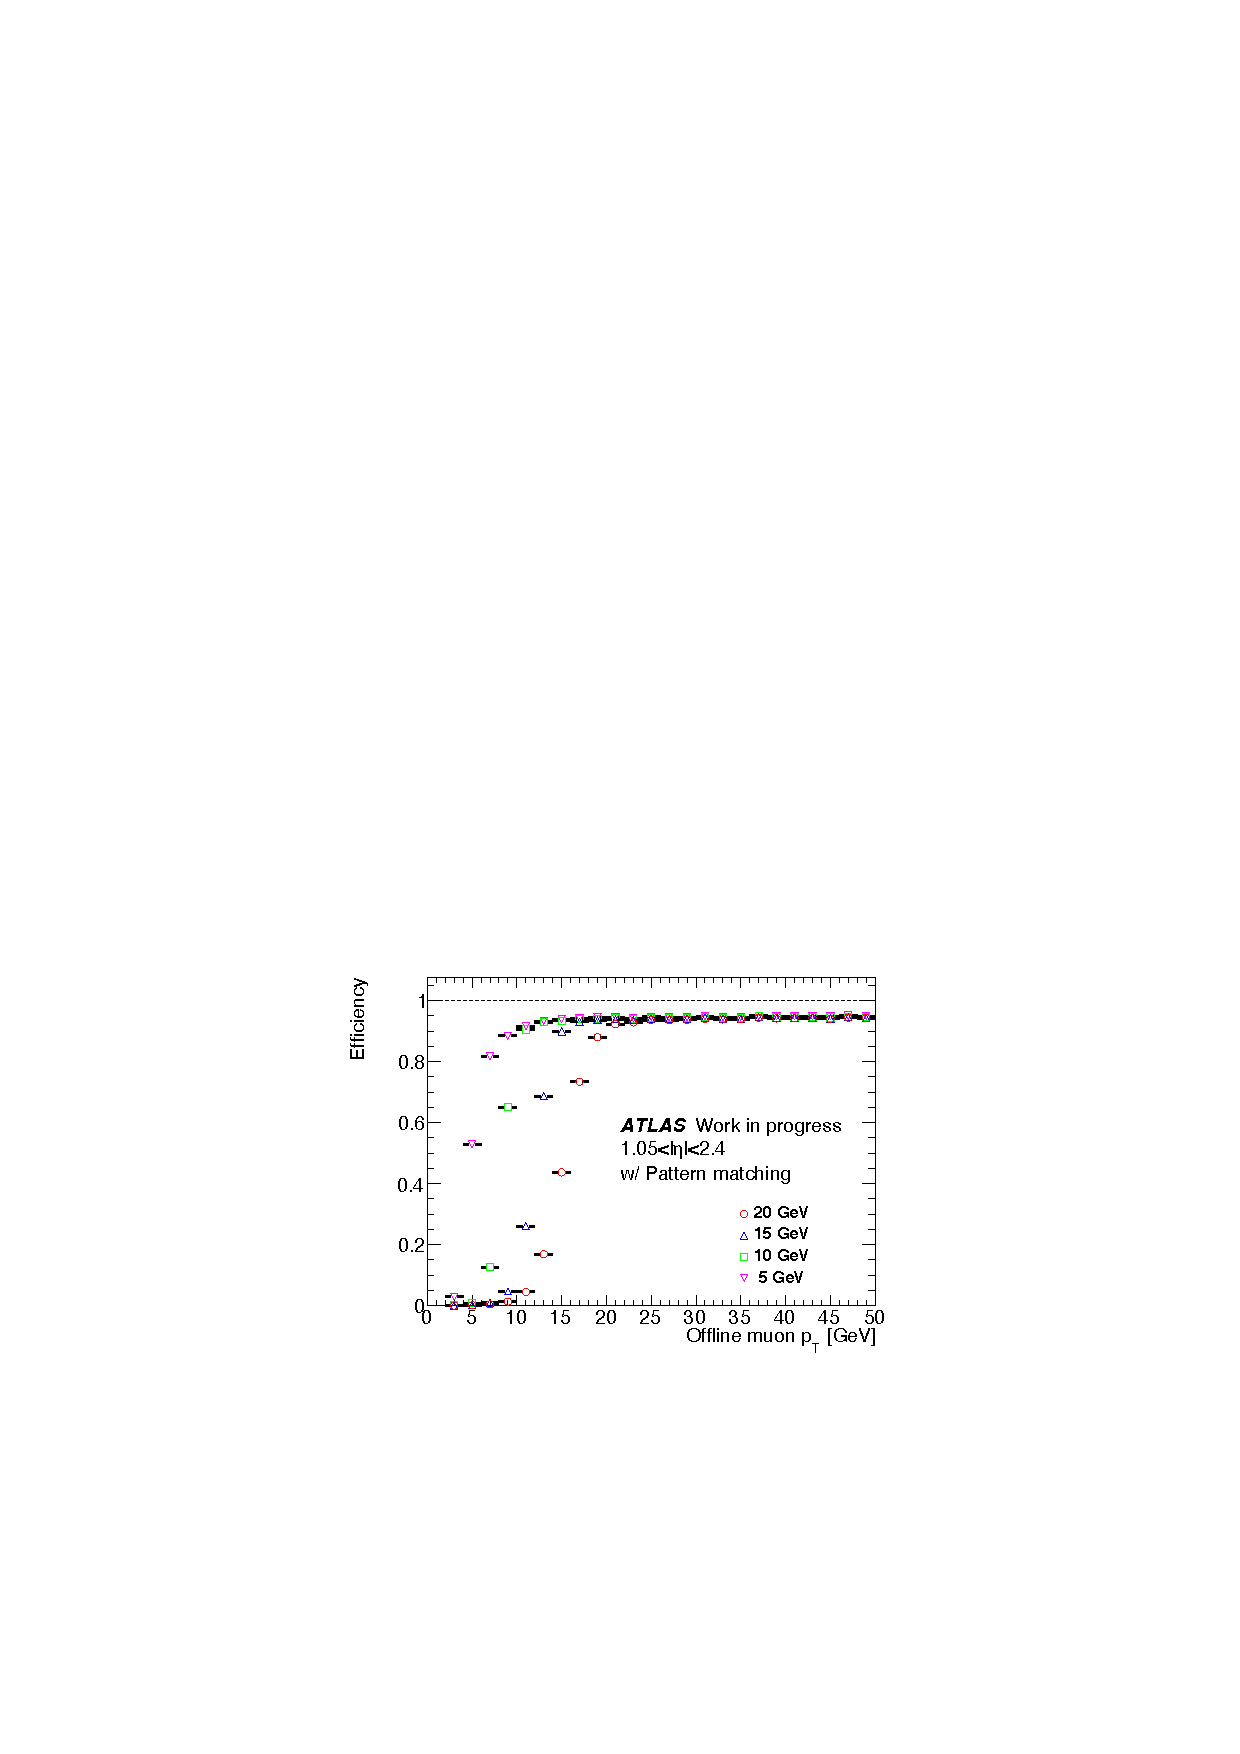
\includegraphics[width=16cm]{fig/Test/Soft_WS.pdf}
    \caption[ソフトウェアシミュレーターで測定された、Wire Strip Coincidenceのトリガー効率]{ソフトウェアシミュレーターで測定された、Wire Strip Coincidenceのトリガー効率\cite{SLPDR}。20 < $p_\mathrm{T}$のプラトー領域でのefficiencyは94 \%程度である。}
    \label{Soft_WS}
\end{figure}

\subsubsection*{Vivado シミュレーターによるHDLの動作検証}
Vivado シミュレーターで測定された、Single Muon  MC に対する Wire Segment Reconstructionの再構成性効率を図\ref{Vivado_Wire_Efficiency}に示す。この試験でも同様のSingle Muon MCサンプルが利用された。この試験ではMCサンプルに含まれるTGC チェンバーのヒットチャンネル情報を、Wire Station Coincidenceのインプットに適したフォーマットに整形した上でVivadoシミュレーションに入力された。Efficiencyは以下のように定義され、Truth Muonの$\eta$、$\phi$ごとにビンわけされている。

\begin{figure}
    \begin{minipage}[b]{.5\linewidth}
    \centering
    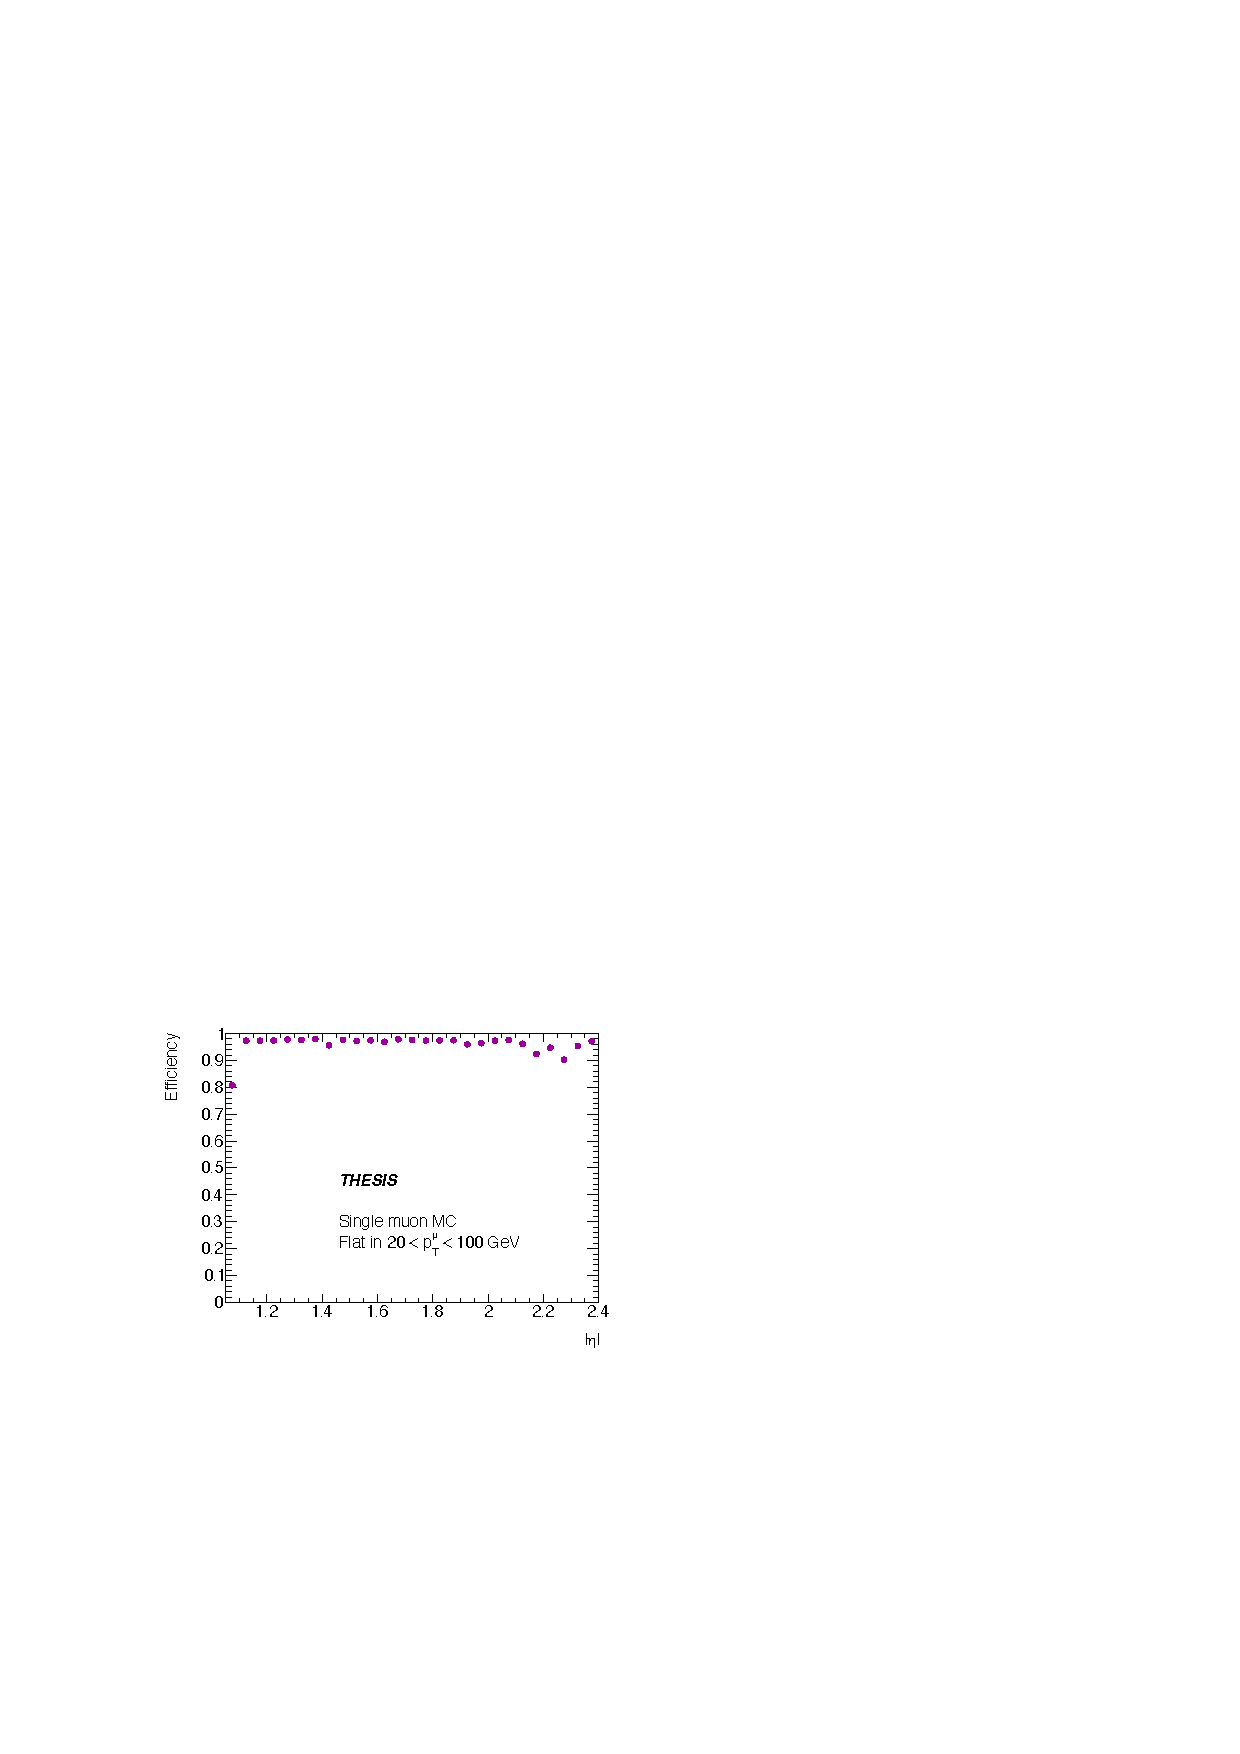
\includegraphics[height=6cm]{fig/Test/Vivado_Wire_eta.pdf}
    \subcaption{Efficiencyの$\eta$依存性}
    \end{minipage}%
    \begin{minipage}[b]{.5\linewidth}
    \centering
    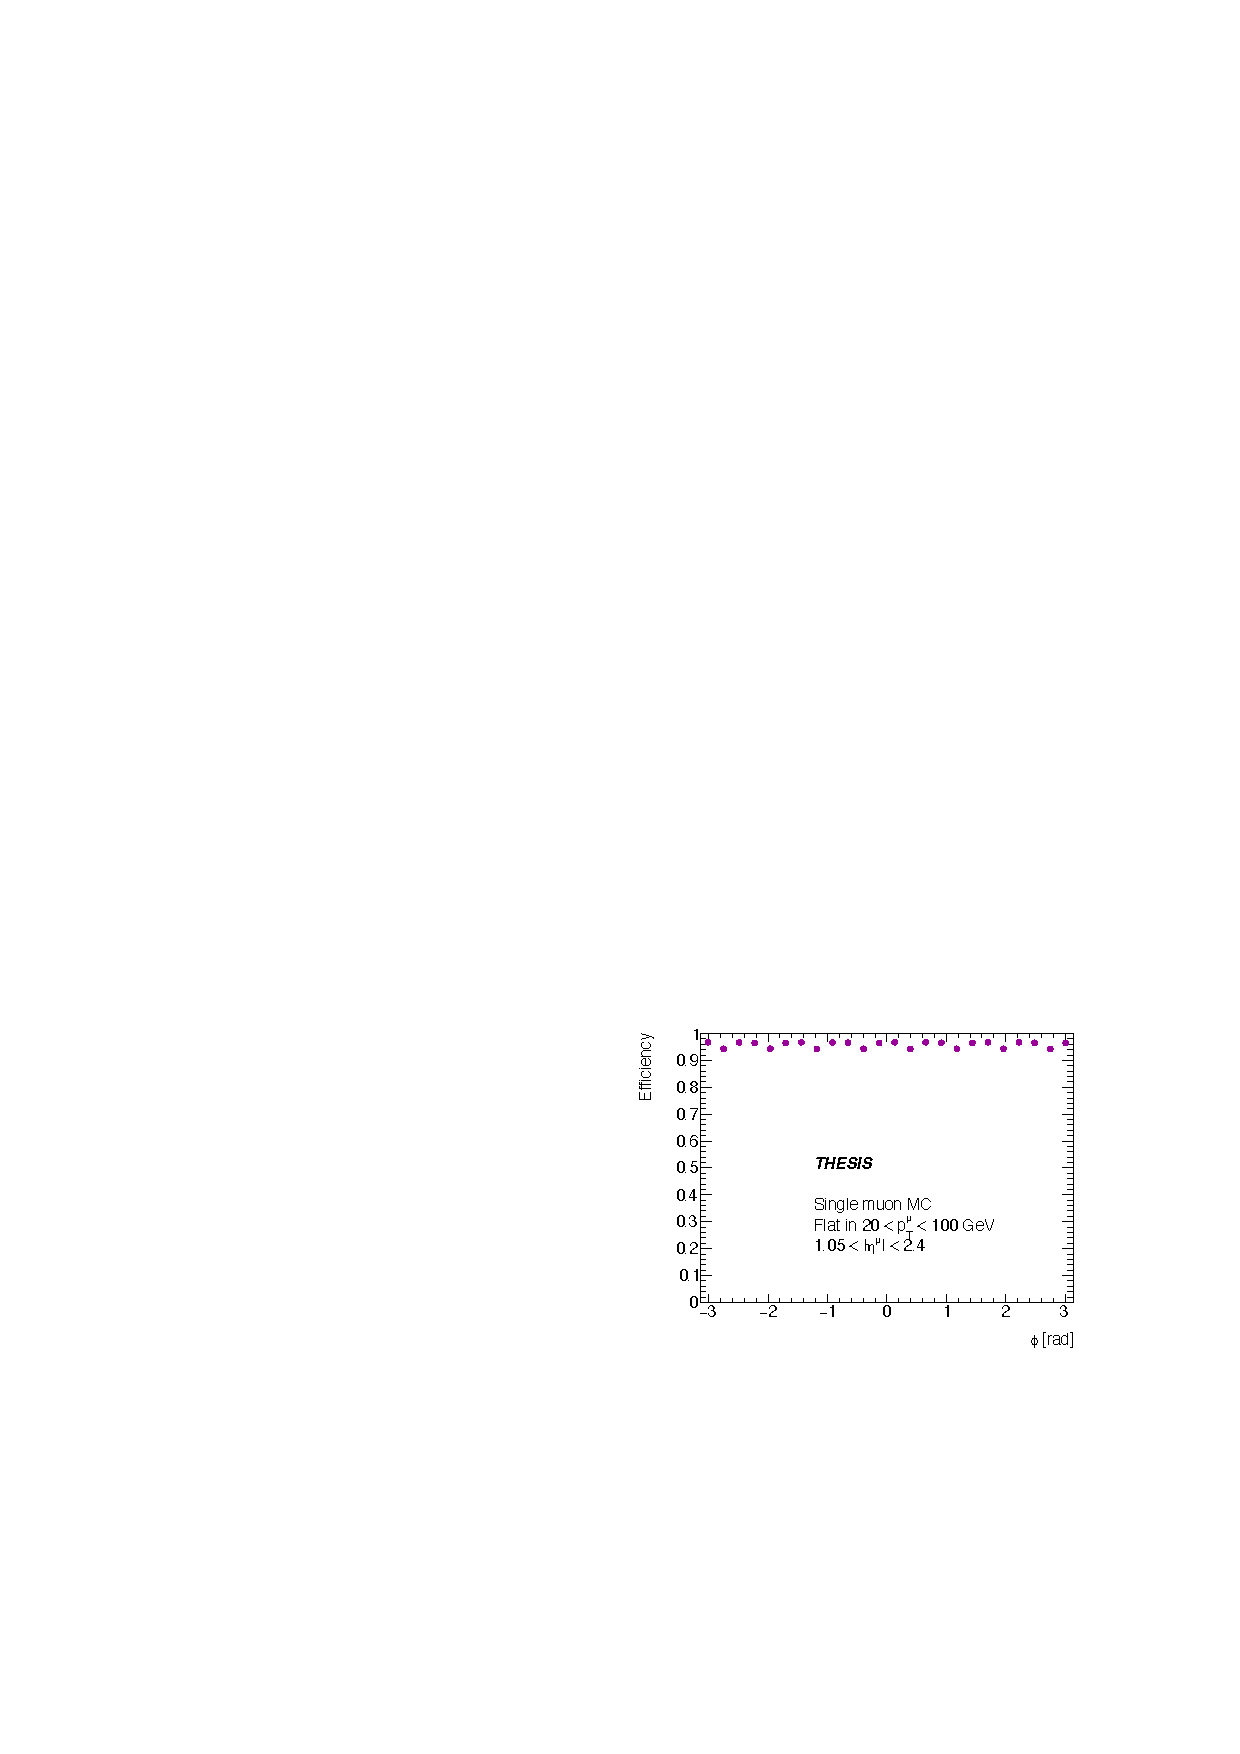
\includegraphics[height=6cm]{fig/Test/Vivado_Wire_phi.pdf}
    \subcaption{Efficiencyの$\phi$依存性}
    \end{minipage}%
    \caption[Wire Segment Reconstructionの検出効率]{Wire Segment Reconstructionの検出効率\cite{mt_nabeyama}。$\eta$、$\phi$全領域でトリガー効率は95 \%程度に達している。}
    \label{Vivado_Wire_Efficiency}
    \end{figure}
    
    \begin{equation}
    \mathrm{Efficiency} = \frac{\mathrm{Wire \,Segment \,Reconstructionで}\,\Delta\theta\,\mathrm{を再構成できたイベント数}}{\mathrm{Truth ミューオン の数}}
\end{equation}

TGCチェンバーの構造やエンドキャップマグネットとの干渉によると考えられる、数\%のInefficiencyが局所的に見られるものの、Efficiencyは$\eta$、$\phi$全領域で95 \%程度に達している。これによりWire Segment ReconstructionのHDL実装が期待通り達成されていることが検証された。

HDL実装された Strip Segment Reconstruction と Wire strip Coincidence の動作検証は、ソフトウェアシミュレーター出力との一致を確かめることで行われた。Strip Segment Reconstruction ではソフトウェアシミュレーターによるStrip Station Coincidenceの出力をVivadoシミュレーターのインプットとし、出力をソフトウェアシミュレーターと比較した。比較結果を表\ref{tab:Vivado_strip}に示す。エンドキャップ領域 (EC) 、フォワード領域 (FW) それぞれで出力の96 \%程度一致した。数\%の不一致は、Segment Reconstructionをパスした飛跡候補が複数あった場合にどれを優先的に後段に送るか、という候補選択ロジックの差異によるものであると理解されている。同じユニット内でヒットレイヤー数が同じ、かつユニット中心からの距離も同じである候補が存在する場合、HDLではM3 スタッガードチャンネルの上位bitを優先に選ぶ、というロジックが実装されているが、ソフトウェアシミュレーターではその二つを仕分ける方法が用意されていない。

\begin{table}[]
    \centering
    \caption{Strip Segment Reconstruction出力のソフトウェアシミュレーターとVivadoシミュレーター比較結果。ECはエンドキャップ領域、FWはフォワード領域を示す。\cite{mt_kawamoto}}
    \label{tab:Vivado_strip}
    \begin{tabular}{|c|cc|}
    \hline
    \multirow{2}{*}{}        & \multicolumn{2}{c|}{割合}                \\ \cline{2-3} 
                             & \multicolumn{1}{c|}{EC}      & FW      \\ \hline\hline
    飛跡情報が一致したイベント            & \multicolumn{1}{c|}{96.8 \%} & 97.8 \% \\ \hline
    候補の選び方の違いに由来する差異があったイベント & \multicolumn{1}{c|}{3.2 \%}  & 2.2 \%  \\ \hline
    候補の選び方以外に由来する差異があったイベント  & \multicolumn{1}{c|}{1.8 \%}  & 0 \%    \\ \hline
    \end{tabular}
\end{table}

Wire Strip Coincidenceの動作検証では、ソフトウェアシミュレーターによるWire Segment ReconstructionとStrip Segment Reconstructionの出力を取り出して、Vivadoシミュレーターのインプットとした。比較結果を表\ref{tab:Vivado_WS}に示す。同様のわずかなロジックの違いによる出力の不一致は存在するが、概ねソフトウェアで設計されたロジックと同等のものをHDLで実装できていることが確認された。

\begin{table}[]
    \centering
    \caption{Wire Strip Coincidence出力のソフトウェアシミュレーターとVivadoシミュレーター比較結果。ECはエンドキャップ領域、FWはフォワード領域を示す。\cite{mt_kawamoto}}
    \label{tab:Vivado_WS}
    \begin{tabular}{|c|cc|}
    \hline
    \multirow{2}{*}{}                      & \multicolumn{2}{c|}{割合}                \\ \cline{2-3} 
                                           & \multicolumn{1}{c|}{EC}      & FW      \\ \hline\hline
    飛跡情報が一致したイベント                          & \multicolumn{1}{c|}{98.4 \%} & 99.9 \% \\ \hline
    飛跡情報の異なったイベント                          & \multicolumn{1}{c|}{1.6 \%}  & 0.07 \% \\ \hline
    イベントで最大の\textbackslash{}pt出力がことなったイベント & \multicolumn{1}{c|}{0.09 \%} & 0.02 \% \\ \hline
    \end{tabular}
\end{table}



\clearpage


\section{タイミングバイオレーションへの対処}
\label{sec:appendix:timing_violation}
Inner Coincidenceを統合した当初はタイミング違反が発生した。本節ではタイミング違反解決までに行った2種類の最適化について説明する。

Inner Coincidenceを統合した後のデバイスのリソース使用状況を表\ref{tab:Resource_before}に示す。表中の値は、1つのSLR中のリソースに対する使用量の割合を百分率で表したものである。Totalにはトリガーロジックだけでなく、コントロール、リードアウトのロジックも含めたリソース使用状況を示している。
BRAMやURAMなどのメモリーデバイスには余裕を持って実装できている一方で、Inner Coincidenceを統合したSLR1ではConfigurable Logic Block (CLB) の使用率が100 \%に達しており、リソースが逼迫している。SLのファームウェアはまだ開発段階であり、機能が増築されていくことを考えるとリソースの削減が必要不可欠であることが判明した。
\begin{table}[]
    \centering
    \caption{Inner Coincidenceを統合した後のデバイスのリソース使用状況}
    \label{tab:Resource_before}
    \begin{tabular}{|c|c|c|c|c|c|c|c|}
    \hline
    Name                                                                        & Block                        & \begin{tabular}[c]{@{}c@{}}LUT \\ (17280000)\end{tabular} & \begin{tabular}[c]{@{}c@{}}REG \\ (34560000)\end{tabular} & \begin{tabular}[c]{@{}c@{}}CLB \\ (2160000)\end{tabular} & \begin{tabular}[c]{@{}c@{}}LUT as Memory \\ (791040)\end{tabular} & \begin{tabular}[c]{@{}c@{}}BRAM \\ (2688)\end{tabular} & \begin{tabular}[c]{@{}c@{}}URAM\\  (1280)\end{tabular} \\ \hline\hline
    \multirow{6}{*}{\begin{tabular}[c]{@{}c@{}}SLR0 \\ EC $\phi$1\end{tabular}} & Wire Station Coincidence     & 7.4                                                       & 1.48                                                      & 22.2                                                     & 0                                                                 & 0                                                      & 0                                                      \\ \cline{2-8} 
                                                                                & Strip Station Coincidence    & 0                                                         & 0.2                                                       & 0.96                                                     & 0                                                                 & 0                                                      & 0                                                      \\ \cline{2-8} 
                                                                                & Wire Segment Reconstruction  & 16.28                                                     & 2.96                                                      & 28.12                                                    & 0                                                                 & 0                                                      & 45.88                                                  \\ \cline{2-8} 
                                                                                & Strip Segment Reconstruction & 6.24                                                      & 3.08                                                      & 11.04                                                    & 0.08                                                              & 0                                                      & 2.43                                                   \\ \cline{2-8} 
                                                                                & Wire Strip Coincidence       & 3.56                                                      & 3.76                                                      & 14.56                                                    & 0                                                                 & 37.52                                                  & 0                                                      \\ \cline{2-8} 
                                                                                & Total                        & 58.24                                                     & 31.04                                                     & 95.28                                                    & 1.08                                                              & 73.68                                                  & 51.56                                                  \\ \hline\hline
    \multirow{3}{*}{SLR1}                                                       & Inner Coincidence            & 67.8                                                      & 19                                                        & 83.64                                                    & 3                                                                 & 28.88                                                  & 50                                                     \\ \cline{2-8} 
                                                                                & Track Selector               & 15.4                                                      & 1.76                                                      & 17.72                                                    & 0                                                                 & 0                                                      & 0                                                      \\ \cline{2-8} 
                                                                                & Total                        & 87.16                                                     & 45.24                                                     & 100                                                      & 3                                                                 & 28.88                                                  & 50                                                     \\ \hline\hline
    \multirow{6}{*}{\begin{tabular}[c]{@{}c@{}}SLR2 \\ EC $\phi$1\end{tabular}} & Wire Station Coincidence     & 7.4                                                       & 1.48                                                      & 22.2                                                     & 0                                                                 & 0                                                      & 0                                                      \\ \cline{2-8} 
                                                                                & Strip Station Coincidence    & 0                                                         & 0.2                                                       & 0.96                                                     & 0                                                                 & 0                                                      & 0                                                      \\ \cline{2-8} 
                                                                                & Wire Segment Reconstruction  & 16.28                                                     & 2.96                                                      & 28.12                                                    & 0                                                                 & 0                                                      & 45.88                                                  \\ \cline{2-8} 
                                                                                & Strip Segment Reconstruction & 6.24                                                      & 3.08                                                      & 11.04                                                    & 0.08                                                              & 0                                                      & 2.43                                                   \\ \cline{2-8} 
                                                                                & Wire Strip Coincidence       & 3.56                                                      & 3.76                                                      & 14.56                                                    & 0                                                                 & 37.52                                                  & 0                                                      \\ \cline{2-8} 
                                                                                & Total                        & 58.24                                                     & 31.04                                                     & 95.28                                                    & 1.08                                                              & 73.68                                                  & 51.56                                                  \\ \hline\hline
    \multirow{6}{*}{\begin{tabular}[c]{@{}c@{}}SLR3 \\ FW\end{tabular}}         & Wire Station Coincidence     & 3.84                                                      & 0.64                                                      & 8.96                                                     & 0                                                                 & 0                                                      & 0                                                      \\ \cline{2-8} 
                                                                                & Strip Station Coincidence    & 0                                                         & 0.04                                                      & 0.16                                                     & 0                                                                 & 0                                                      & 0                                                      \\ \cline{2-8} 
                                                                                & Wire Segment Reconstruction  & 6.4                                                       & 1.28                                                      & 9.6                                                      & 0                                                                 & 0                                                      & 19.84                                                  \\ \cline{2-8} 
                                                                                & Strip Segment Reconstruction & 1.24                                                      & 0.6                                                       & 2.52                                                     & 0.04                                                              & 0                                                      & 1.24                                                   \\ \cline{2-8} 
                                                                                & Wire Strip Coincidence       & 1.52                                                      & 1.6                                                       & 5.36                                                     & 0                                                                 & 14.28                                                  & 0                                                      \\ \cline{2-8} 
                                                                                & Total                        & 25.84                                                     & 15.88                                                     & 52.04                                                    & 0.48                                                              & 32.52                                                  & 20.32                                                  \\ \hline
    \end{tabular}
\end{table}

タイミングの解析の結果を表\ref{tab:timing_before}に示す。
Setup解析、Hold解析どちらにおいてもタイミング違反 (タイミングバイオレーション) が発生した。本研究では特に、Total Negative Slack (TNS) をタイミング違反の定量化に利用する。TNSとは、FPGA内に含まれる全てのフリップフロップパス間のネガティブスラックを足し上げたもので、どれだけタイミング深刻なタイミング違反かということと (Worst Negative Slack , WNS) と、どれだけ広範囲にタイミング違反が生じているか ( Number of Failing EndPoints )どちらにも相関を持つ値となっている。タイミング違反が発生した場合には負の値をとる。タイミングバイオレーションが生じている場合、ファームウェアの正常動作は保証されないため、これに関しても改善が必要である。
\begin{table}[]
    \centering
    \caption{Inner Coincidence統合後のタイミング解析の結果}
    \label{tab:timing_before}
    \begin{tabular}{|c|c|c|}
    \hline
    Name                                                    & Setup         & Hold        \\ \hline\hline
    Worst Negative Slack (WNS) / Worst Hold Slack (WHS)     & -8.616 ns     & -0.256 ns   \\ \hline
    Number of Failing Endpoints / Total Number of Endpoints & 59 K / 1911 K & 9K / 1911 K \\ \hline
    Total Negative Slack (TNS) / Total Hold slack           & -126, 297 ns  & -388 ns     \\ \hline
    \end{tabular}
\end{table}

本節ではInner Coincidenceを統合したことにより生じたタイミングバイオレーションを解決するために行った2つの最適化について説明する。いずれも、FPGAで実現される論理自体に変更を加えることなく、リソースの使い方を最適化したものであり、トリガーロジックの性能に影響を与えるものではない。

\subsection{シフトレジスタ実装方法の最適化}
タイミングバイオレーション問題の解決に向けて、まずシフトレジスターの実装方法を検討した。
一般に、FPGAでタイミング違反が生じた場合、2つのフリップフロップ間にシフトレジスターを挟む処理が行われる。これは、回路の大規模化に伴ってフリップフロップが離れた位置に配置された場合でも、シフトレジスたを挟むことで、フリップフロップ間の距離が短くなりタイミング制約を緩和することができるからである。この目的で挿入されるシフトレジスタをパイプラインレジスタと呼ぶ。SL FPGAでもこれまでタイミング違反が生じた場合に、この処置がとられて来た。たとえば、Wire Station CoincidenceとWire Segment Reconstructionの間で2段、Wire Segment ReconstructionとWire Strip Coincidenceの間で2段のパイプラインレジスタが挿入されている。

ところで、UltraScale+ FPGAではシフトレジスタを実装するのに2種類のプリミティブ\footnote{FPGAの最小構成要素。FPGAの論理回路はプリミティブの組み合わせで構成される。代表的にはLUT、Flip Flop、RAMなどがある。目的の論理回路を実現するのにどのプリミティブを利用し、FPGA内のどこに配置するかは”Vivado”ソフトウェアで自動で行われる。}が用意されている。それぞれの概要を図\ref{SL_ShiftRegister}に示す。1つ目はD Flip-Flop with Clock Enable and Synchronous Reset (FDRE)と呼ばれる基本的なフリップフロップである。1つのFDREは1 bitのデータを保持するため、width n, depth mのシフトレジスタを実装するにはn x m個のFDREが必要となる。2つ目はShift Register LUT (SRL)と呼ばれる、メモリー用のLUTである。最大のdepthが16のもの(SRL16E) と32 (SRLC32E)のものが存在し、同様のシフトレジスターをSRLC32Eで実現しようとすると n x (m/32)個プリミティブを使用する。

\begin{figure}
\begin{minipage}[b]{.5\linewidth}
\centering
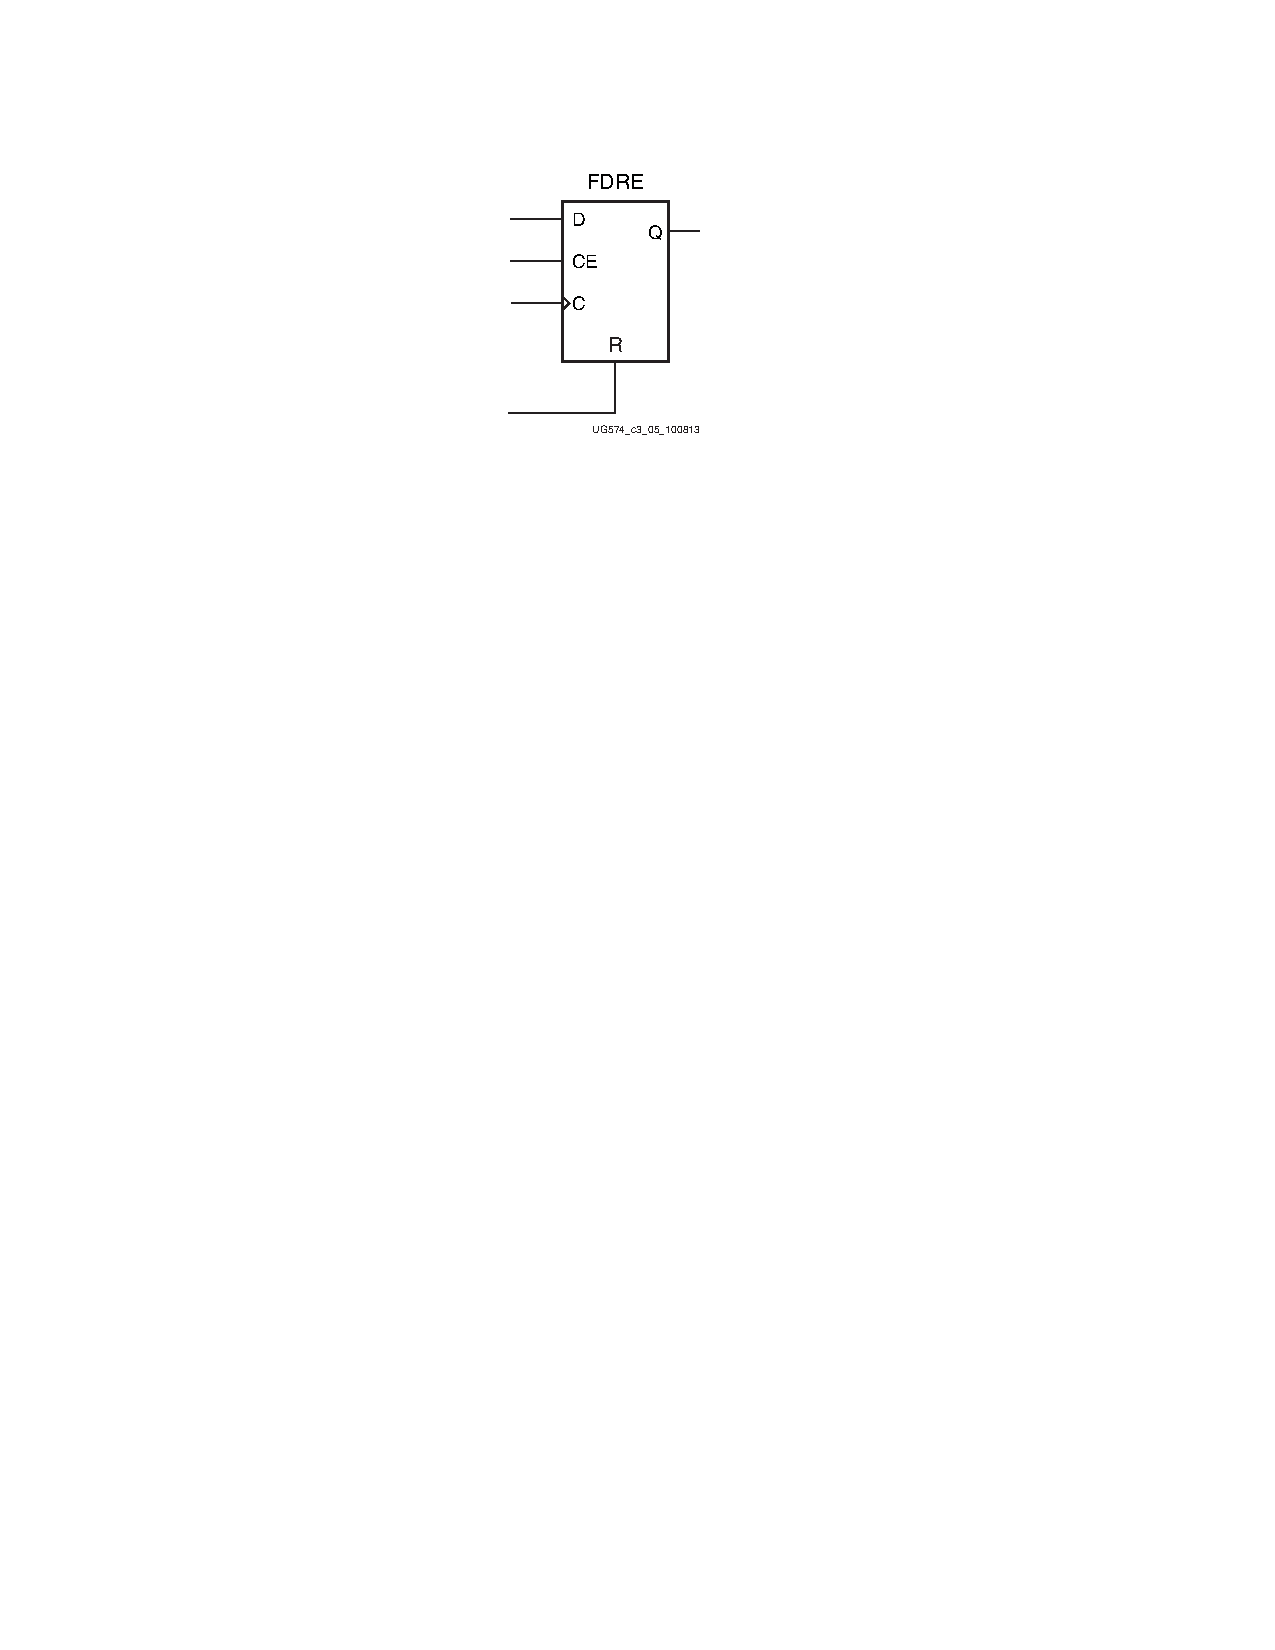
\includegraphics[height=5cm]{fig/SL/FDRE.pdf}
\subcaption{FERE Primitiveのロジックブロック}
\end{minipage}%
\begin{minipage}[b]{.5\linewidth}
\centering
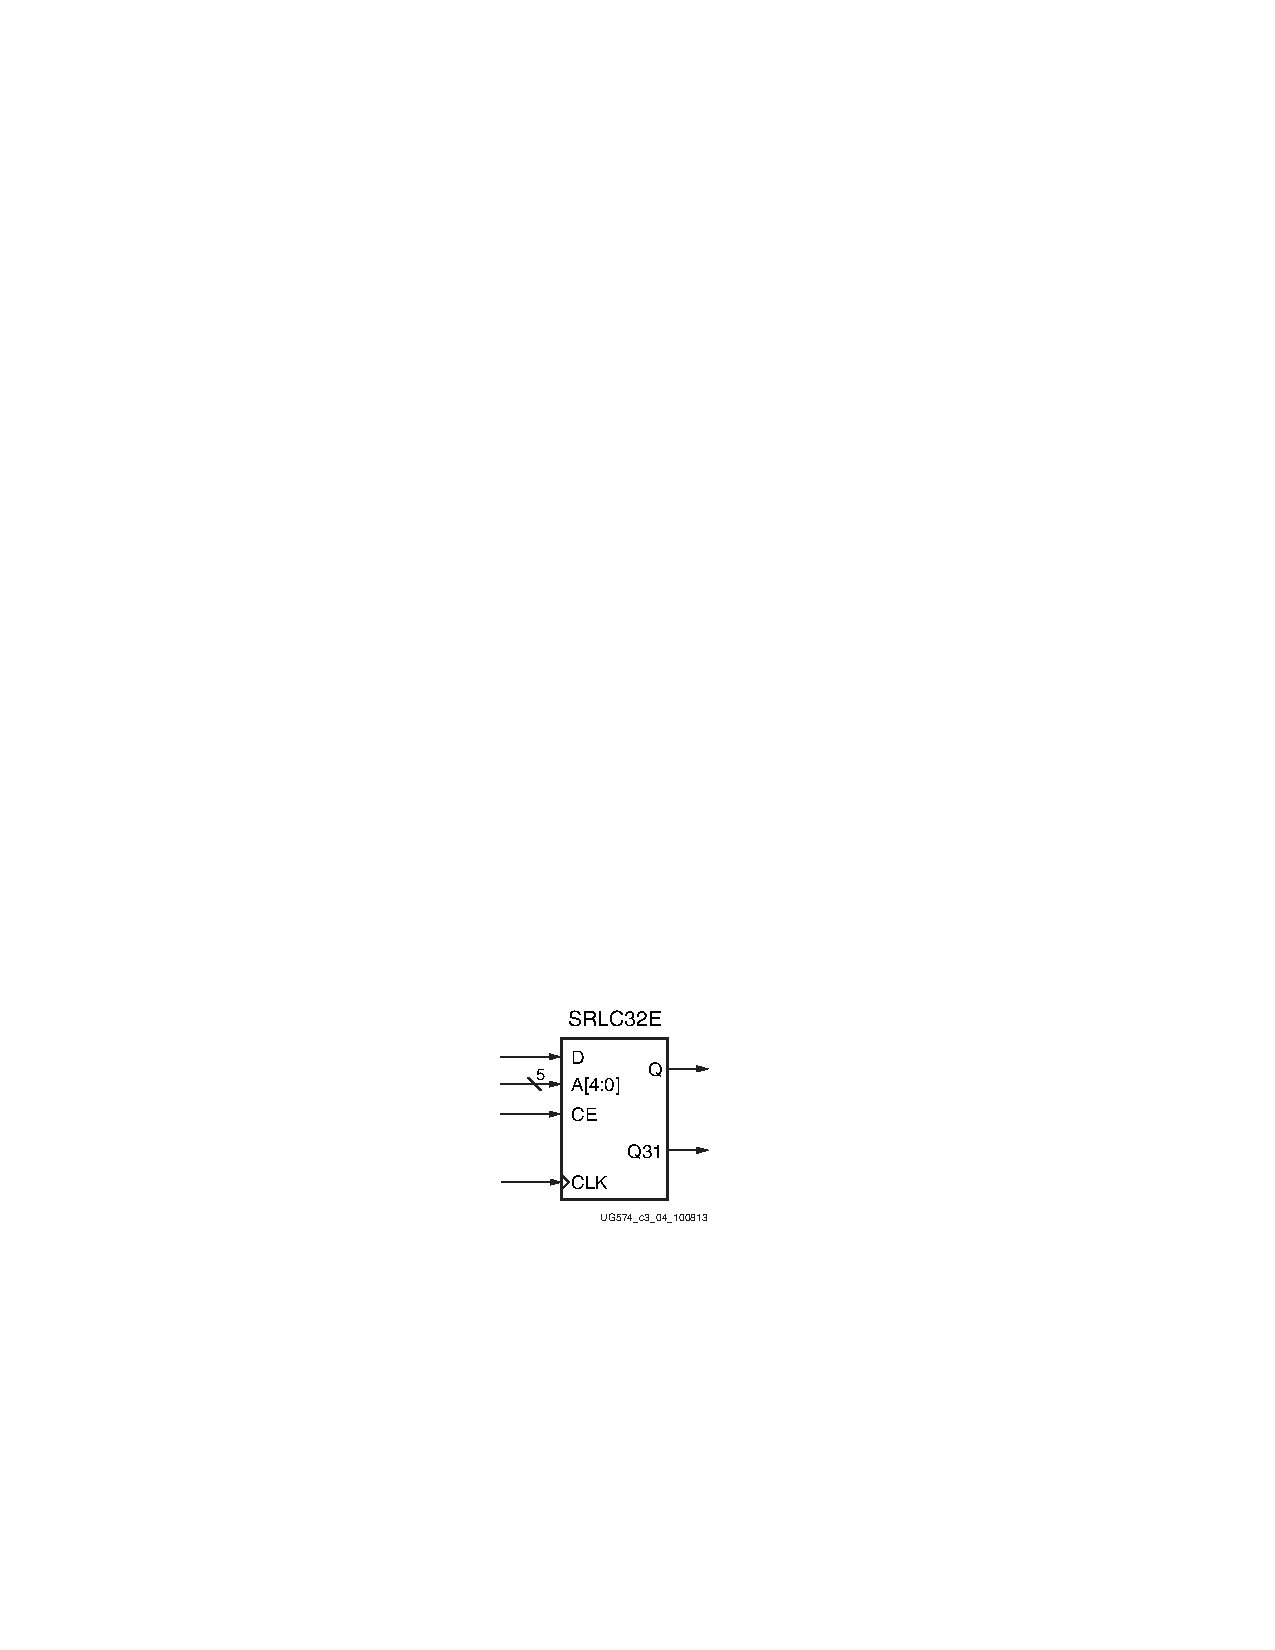
\includegraphics[height=5cm]{fig/SL/SRLC32E.pdf}
\subcaption{SRLC32E Primitiveのロジックブロック}
\end{minipage}%
\caption[シフトレジスタを構成するプリミティブ]{異シフトレジスタを構成するプリミティブ\cite{UltraScale_Architecture}}
\label{SL_ShiftRegister}
\end{figure}

これまでSL FPGAではパイプラインレジスタを実現するのにFDREのみを利用していた。これは一連のシフトレジスタがが1つのSRLタイルに配置されると、ロジックとロジックを繋ぐ中継点の役割を果たさず、タイミング制約を緩和するという本来の役割を果たさなくなると考えられていたからである。しかし、ロジックが大規模になり、基本的なプリミティブであるFDREの使用量が増えてくるとFPGA内に密集が発生し、逆に適切な位置にパイプラインレジスタを配置できなくなることも考えられる。そこで、本研究ではFDREに加えてSRLも利用してimplemetationを行い、どちらの方がタイミング制約の緩和に有効な実装方法か調査した。

図\ref{SRL_FDRE}にSLR0のプリミティブ使用状況を示す。図の黄色のcellがSLR0内のパイプラインレジスタの実装に利用されているプリミティブである。FDREのみを利用した場合、パイプラインレジスタはFDRE 50 K個を用いて実装されている。一方SRLも利用した場合、パイプラインレジスタはSRL 6K、FDRE 6K個を利用して実装される。
図\ref{}に変更前後におけるファームウェア全体でのネガティブスラック発生状況、表\ref{}にタイミング解析の結果を示す。SRLを利用することで、TNSは-126297.769 ns から -7903.744 nsに約1/16に削減された。この結果は、SRLを使うと、フリップフロップ間の距離が遠いところには適切にパイプラインを設置し、逆に近いところでは数段のパイプラインをまとめてSRLに実装するなど、より柔軟なロジックの配置が実現したことによるものと考えられる。
しかし依然としてタイミングバイオレーションは解決しておらず、さらなる改善が求められる。

\begin{figure} 
\centering
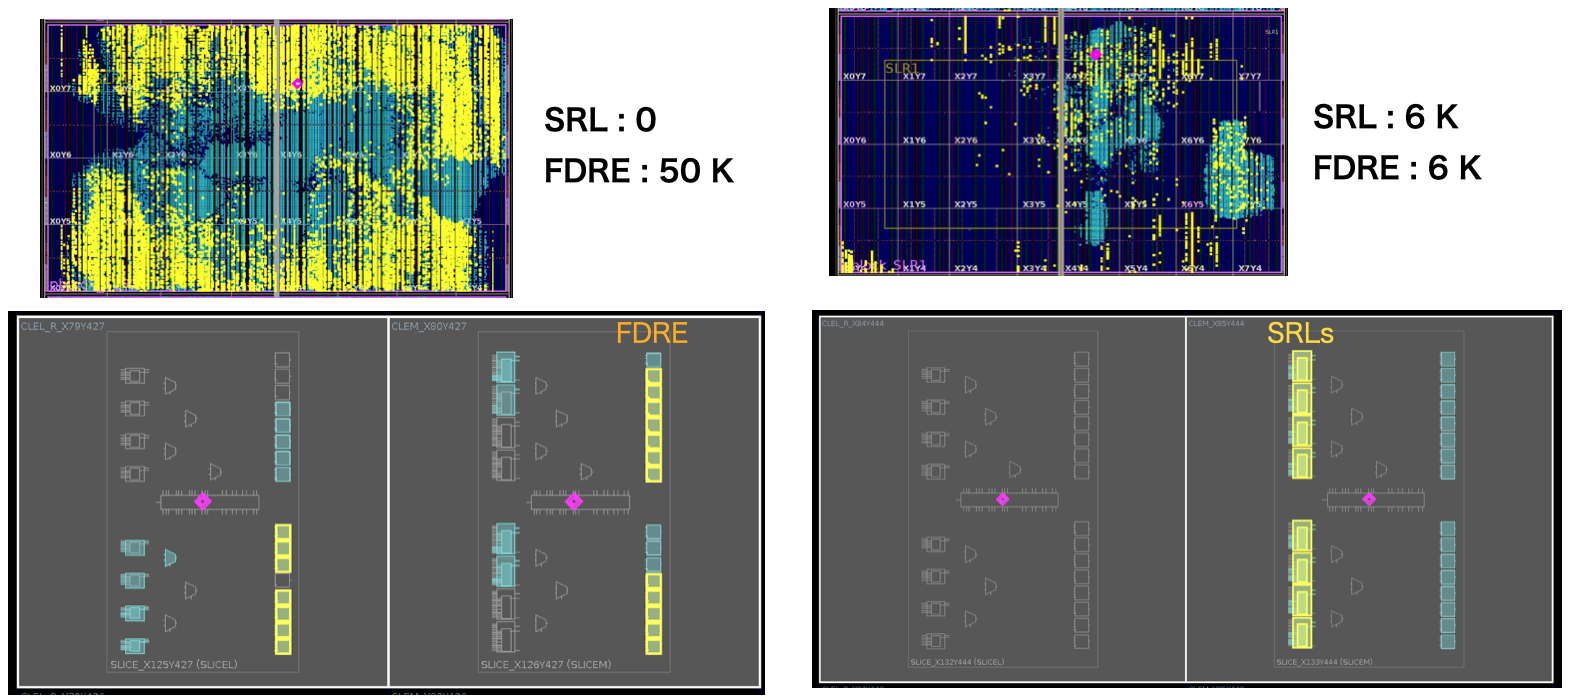
\includegraphics[width=16cm]{fig/SL/SRL_FERE.png}
\caption[SRLを利用する場合と利用しない場合におけるリソース使用状況の比較]{SRLを利用する場合と利用しない場合におけるリソース使用状況の比較}
\label{SRL_FDRE}
\end{figure}


\subsection{Track Selectorの最適化}
モジュールごとのネガティブスラックの量をみると、全体の50 \%以上がTrack Selectorで発生しており、トリガーチェーンをタイミング制約を満たして完成させるにはこれの最適化が必要である。そこで本研究ではTrack Selectorにかけるレイテンシーを160 MHz 1チック分増やす代わりに、ソーティングロジックの簡略化を行い、タイミング制約の緩和を図った。
従来のロジックと変更後のロジックの概念図を図\ref{}に示す。Track SelectorはInner Coincidenceから出力された最大128個のミューオン飛跡候補から、\pt の大きいものを8個選び出すものである。1つのミューオン候補に対して124 bitの情報が用意される。128個の飛跡候補は160 MHzの1チックごとに1 vs 1で\pt 比較が行われ、合計4チックで8候補まで絞り込まれる。従来のロジックではこのソーティングのロジックにおいて124 bit $\times$ 128 候補のデータを並列に並べた上で、124 bitのデータ同士を並び替えていた。これに対し、変更後のロジックではInner Coincidenceから出力される1候補あたり124 bitのデータのうち、ソーティングに利用する\pt 5 bitの情報だけを取り出し並び替えを行い、そのほかのデータは128個の飛跡候補を識別する 7 bit のIDと共にBRAMに格納しておく。ソーティングが完了し8個の飛跡候補が選ばれたら、そのIDを用いてBRAMからデータを取り出す。
この方法では、ソーティングの後BRAMからデータを取り出すのに160 MHz 1チック分レイテンシーが余計にかかってしまうが、ソーティング必要なデータ量を124 bit $\times$ 128 候補から5 bit $\times$ 128 候補に削減することができる。これにより、FPGAで配線する必要のあるプリミティブを大幅に減らすことができ、タイミング制約の緩和が期待される。

図\ref{SL_Metrics}および表\ref{tab:timing_before_after}に最適化前後のタイミング解析の結果をまとめる。シフトレジスタの最適化後にあった-7903.744 nsのTNSは0になっており、タイミングバイオレーションを解決することができた。


\begin{table}[]
    \centering
    \caption{Track Selectorの最適化前後のタイミング解析の結果}
    \label{tab:timing_before_after1}
    \begin{tabular}{|c||cc||cc||cc|}
    \hline
    \multirow{2}{*}{Name}                                                                              & \multicolumn{2}{c||}{最適化前}                        & \multicolumn{2}{c||}{シフトレジスタ最適化}                 & \multicolumn{2}{c||}{Track Selector最適化}      \\ \cline{2-7}
                                                                                                       & \multicolumn{1}{c|}{Setup}         & Hold        & \multicolumn{1}{c|}{Setup}         & Hold       & \multicolumn{1}{c|}{Setup}      & Hold      \\ \hline
    Worst  Slack                                                                                       & \multicolumn{1}{c|}{-8.616 ns}     & -0.256 ns   & \multicolumn{1}{c|}{- 1.164 ns}    & 0          & \multicolumn{1}{c|}{0}          & 0         \\ \hline
    \begin{tabular}[c]{@{}c@{}}Number of Failing Endpoints / \\ Total Number of Endpoints\end{tabular} & \multicolumn{1}{c|}{59 K / 1911 K} & 9K / 1911 K & \multicolumn{1}{c|}{14 K / 1643 K} & 0 / 1643 K & \multicolumn{1}{c|}{0 / 1716 K} & 0 /1716 K \\ \hline
    Total Slack                                                                                        & \multicolumn{1}{c|}{-126, 297 ns}  & -388 ns     & \multicolumn{1}{c|}{- 7903.744}    & 0          & \multicolumn{1}{c|}{0}          & 0         \\ \hline
    \end{tabular}
\end{table}

\begin{figure}
\begin{minipage}[b]{.33\linewidth}
\centering
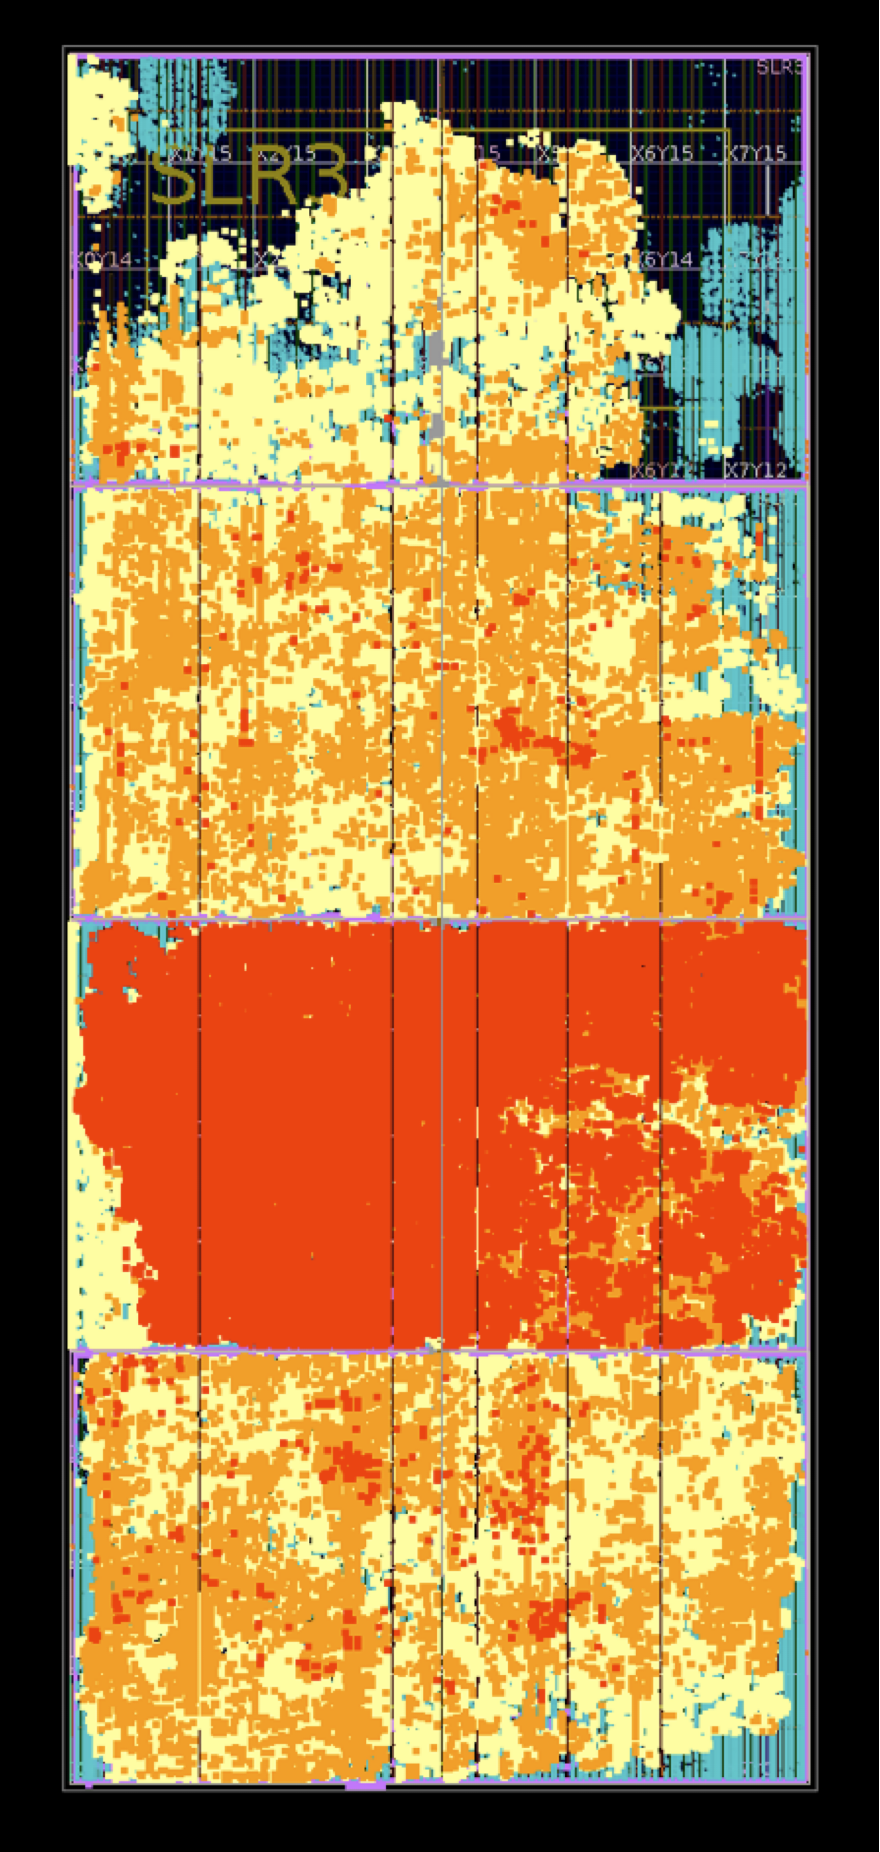
\includegraphics[height=12cm]{fig/SL/Metrics_before.png}
\subcaption{最適化前}
\end{minipage}%
\begin{minipage}[b]{.33\linewidth}
\centering
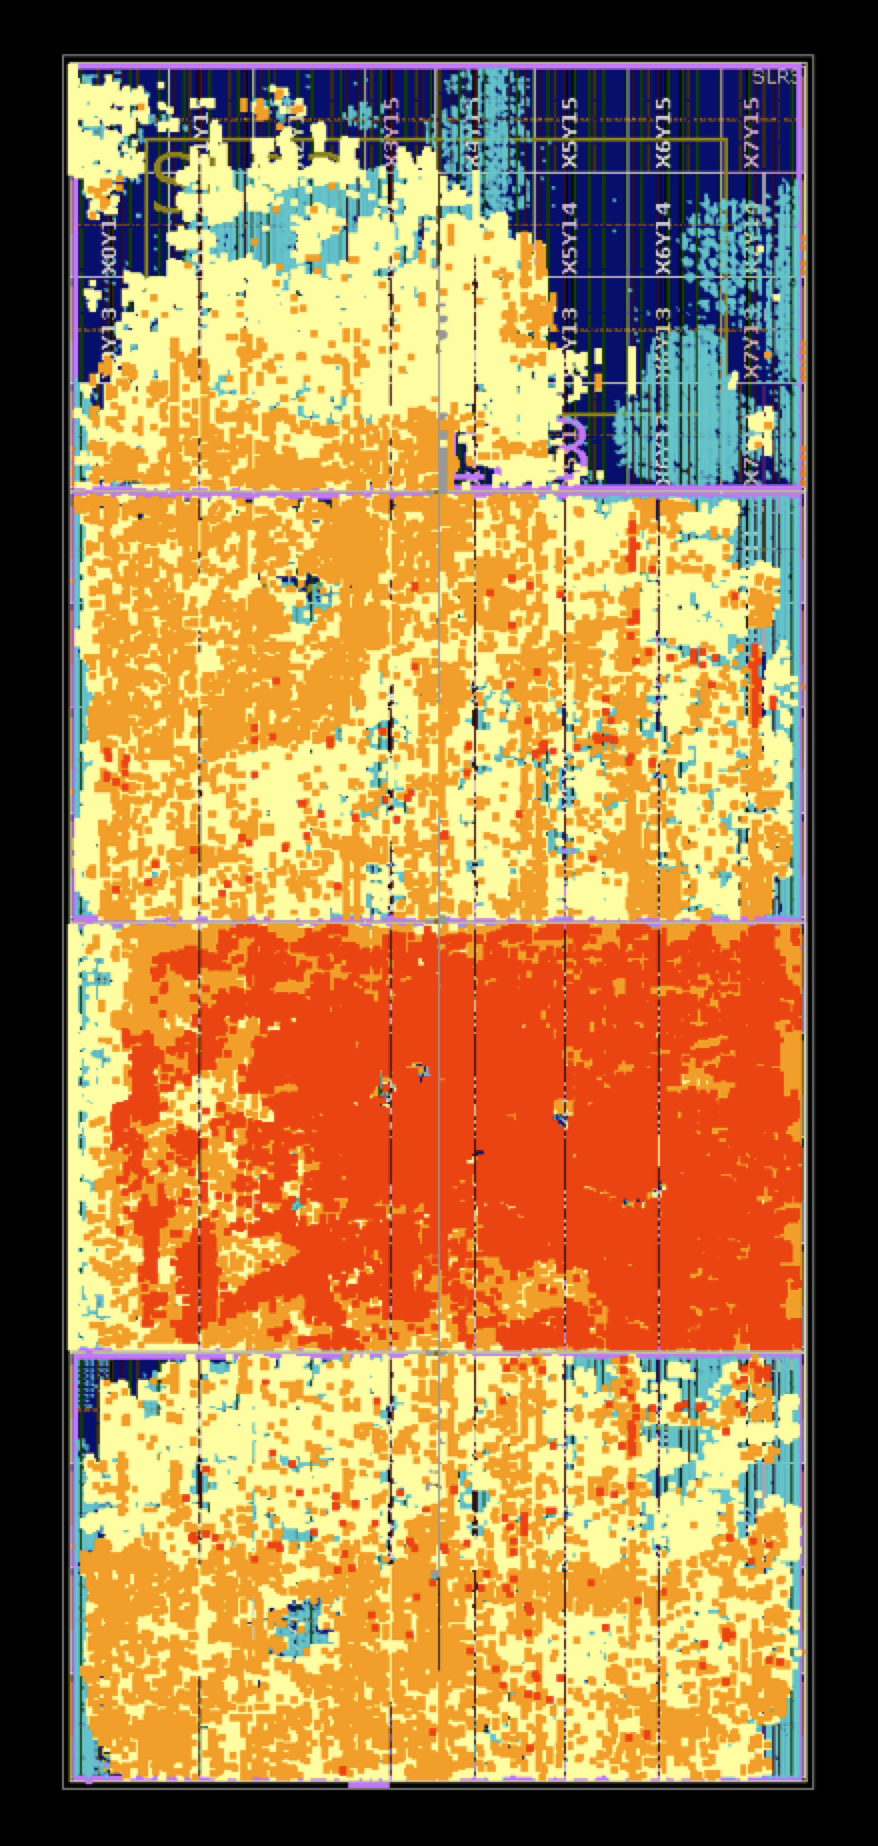
\includegraphics[height=12cm]{fig/SL/Metrics_shiftreg.png}
\subcaption{シフトレジスタ最適化後}
\end{minipage}%
\begin{minipage}[b]{.33\linewidth}
\centering
\includegraphics[height=12cm]{fig/SL/Metrics_trackselector.png}
\subcaption{Track Selector最適化後}
\end{minipage}%
\caption[]{最適化前後のネガティブスラック発生状況。赤色のセルがネガティブスラックが発生している領域を示す。オレンジ、黄色、白色の順に正のスラックが大きい。シフトレジスタの最適化とTrack Selectorの最適化を経て、タイミングバイオレーションを解決することができた。}
\label{SL_Metrics}
\end{figure}

また、最適化後のリソース使用状況を図\ref{tab:Resource_after}に示す。

\begin{table}[]
    \centering
    \caption{最適化後のデバイスのリソース使用状況}
    \label{tab:Resource_after}
    \begin{tabular}{|c|c|c|c|c|c|c|c|}
    \hline
    Name                                                                        & Block                        & \begin{tabular}[c]{@{}c@{}}LUT \\ (17280000)\end{tabular} & \begin{tabular}[c]{@{}c@{}}REG \\ (34560000)\end{tabular} & \begin{tabular}[c]{@{}c@{}}CLB \\ (2160000)\end{tabular} & \begin{tabular}[c]{@{}c@{}}LUT as Memory \\ (791040)\end{tabular} & \begin{tabular}[c]{@{}c@{}}BRAM \\ (2688)\end{tabular} & \begin{tabular}[c]{@{}c@{}}URAM\\  (1280)\end{tabular} \\ \hline\hline
    \multirow{6}{*}{\begin{tabular}[c]{@{}c@{}}SLR0 \\ EC $\phi$1\end{tabular}} & Wire Station Coincidence     & 7.4                                                       & 1.48                                                      & 22.2                                                     & 0                                                                 & 0                                                      & 0                                                      \\ \cline{2-8} 
                                                                                & Strip Station Coincidence    & 0                                                         & 0.2                                                       & 0.96                                                     & 0                                                                 & 0                                                      & 0                                                      \\ \cline{2-8} 
                                                                                & Wire Segment Reconstruction  & 16.28                                                     & 2.96                                                      & 28.12                                                    & 0                                                                 & 0                                                      & 45.88                                                  \\ \cline{2-8} 
                                                                                & Strip Segment Reconstruction & 6.24                                                      & 3.08                                                      & 11.04                                                    & 0.08                                                              & 0                                                      & 2.43                                                   \\ \cline{2-8} 
                                                                                & Wire Strip Coincidence       & 3.56                                                      & 3.76                                                      & 14.56                                                    & 0                                                                 & 37.52                                                  & 0                                                      \\ \cline{2-8} 
                                                                                & Total                        & 58.24                                                     & 31.04                                                     & 95.28                                                    & 1.08                                                              & 73.68                                                  & 51.56                                                  \\ \hline\hline
    \multirow{3}{*}{SLR1}                                                       & Inner Coincidence            & 67.8                                                      & 19                                                        & 83.64                                                    & 3                                                                 & 28.88                                                  & 50                                                     \\ \cline{2-8} 
                                                                                & Track Selector               & 15.4                                                      & 1.76                                                      & 17.72                                                    & 0                                                                 & 0                                                      & 0                                                      \\ \cline{2-8} 
                                                                                & Total                        & 87.16                                                     & 45.24                                                     & 100                                                      & 3                                                                 & 28.88                                                  & 50                                                     \\ \hline\hline
    \multirow{6}{*}{\begin{tabular}[c]{@{}c@{}}SLR2 \\ EC $\phi$1\end{tabular}} & Wire Station Coincidence     & 7.4                                                       & 1.48                                                      & 22.2                                                     & 0                                                                 & 0                                                      & 0                                                      \\ \cline{2-8} 
                                                                                & Strip Station Coincidence    & 0                                                         & 0.2                                                       & 0.96                                                     & 0                                                                 & 0                                                      & 0                                                      \\ \cline{2-8} 
                                                                                & Wire Segment Reconstruction  & 16.28                                                     & 2.96                                                      & 28.12                                                    & 0                                                                 & 0                                                      & 45.88                                                  \\ \cline{2-8} 
                                                                                & Strip Segment Reconstruction & 6.24                                                      & 3.08                                                      & 11.04                                                    & 0.08                                                              & 0                                                      & 2.43                                                   \\ \cline{2-8} 
                                                                                & Wire Strip Coincidence       & 3.56                                                      & 3.76                                                      & 14.56                                                    & 0                                                                 & 37.52                                                  & 0                                                      \\ \cline{2-8} 
                                                                                & Total                        & 58.24                                                     & 31.04                                                     & 95.28                                                    & 1.08                                                              & 73.68                                                  & 51.56                                                  \\ \hline\hline
    \multirow{6}{*}{\begin{tabular}[c]{@{}c@{}}SLR3 \\ FW\end{tabular}}         & Wire Station Coincidence     & 3.84                                                      & 0.64                                                      & 8.96                                                     & 0                                                                 & 0                                                      & 0                                                      \\ \cline{2-8} 
                                                                                & Strip Station Coincidence    & 0                                                         & 0.04                                                      & 0.16                                                     & 0                                                                 & 0                                                      & 0                                                      \\ \cline{2-8} 
                                                                                & Wire Segment Reconstruction  & 6.4                                                       & 1.28                                                      & 9.6                                                      & 0                                                                 & 0                                                      & 19.84                                                  \\ \cline{2-8} 
                                                                                & Strip Segment Reconstruction & 1.24                                                      & 0.6                                                       & 2.52                                                     & 0.04                                                              & 0                                                      & 1.24                                                   \\ \cline{2-8} 
                                                                                & Wire Strip Coincidence       & 1.52                                                      & 1.6                                                       & 5.36                                                     & 0                                                                 & 14.28                                                  & 0                                                      \\ \cline{2-8} 
                                                                                & Total                        & 25.84                                                     & 15.88                                                     & 52.04                                                    & 0.48                                                              & 32.52                                                  & 20.32                                                  \\ \hline
    \end{tabular}
\end{table}

\subsection{今後に向けて : TGC BW コインシデンスの飛跡候補数削減}
本研究の最適化の結果、SL FPGAにおけるタイミングバイオレーションは解決した。しかし、リソース使用量やタイミング制約は依然、逼迫している。特にInner CoincidenceやTrack Selectorが実装されているSLR1のリソース使用量には余裕がなく、タイミング違反もここで生じるものが多かった。また、SLファームウェアは今後拡張が進められていく予定で、Inner Coincidenceに関してだけでも、磁場内部飛跡検出器とのインターフェイスや、テストパターンを打ち込む機構など追加実装される。そこで、今後はより抜本的なロジック最適化が必要になると考える。本節では、今後の最適化の方向性について述べる。

今後の最適化において重要なコンセプトは、余裕のあるレイテンシーを活用してミューオン候補を選別するロジックを導入することで、SLR1に実装されるロジックおよびSLRをまたぐ信号線を削減することである。
現状のロジックではWire Strip Coincidenceで選ばれるミューオン候補は180個におよびそのすべてがSLRを跨いでInner Coincidenceに入力される。また、180個の候補を処理するためにInner Coincidenceでは78個の独立したロジックが走っている。しかし、1枚のSLが処理する1/24セクターの1BCの間に、物理的に意味のあるミューオンが大量に入射することは極めて稀である。現状の180個ミューオンが同時に入ってきても処理できるようなシステムは合理的でないと考えられる。図\ref{SL_Trigger_Compare}にRun3と高輝度LHC実験のトリガーロジックをミューオン飛跡候補数の観点でまとめた。どちらもEndcap Phi0の1 トリガーセクターに関するもので、Station間コインシデンスまではWireのロジックにおけるミューオン候補数を示している。Run3のロジックではHPTにおけるステーション間コインシデンスで1 トリガーセクターあたりミューオンの候補数を 7個まで絞り込む。Wire Strip CoincidenceからInner Coincidenceまでも高々 19個のミューオン候補しか渡されない。一方、高輝度LHC実験ではステーション間コインシデンスで最大 148個、Wire Strip CoincindenceからInner Coincidenceで 74個のミューオン候補が渡される。Run3のロジックでも95 \%前後のトリガー効率を達成できていたことを考えると、トリガー効率を損ねることなくミューオン候補数を削減することは可能であると考えられる。

\begin{figure} 
\centering
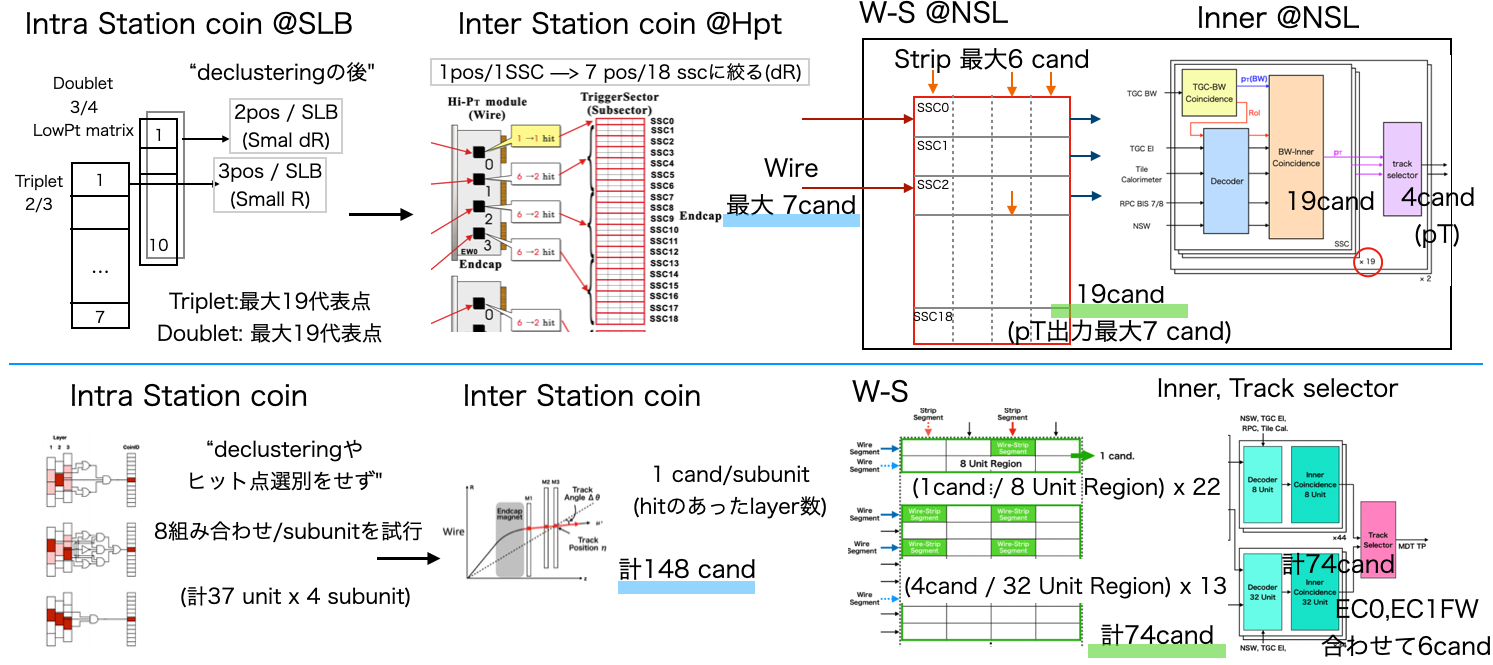
\includegraphics[width=16cm]{fig/SL/Trigger_Compare.png}
\caption[Run3と高輝度LHCのミューオン候補数の比較]{Run3と高輝度LHCのミューオン候補数の比較}
\label{SL_Trigger_Compare}
\end{figure}

また、L0 trigger latencyも2.5 $\mu$sから10 $\mu$sに拡張されたことにより、トリガー判定に使える時間にはまだ十分な余裕がある。図\ref{Trigger_latency_memo}に現状のトリガーロジックのトリガーレイテンシーを示す。陽子バンチ交差を時間の原点にとると、1120 ns後にはWire Strip Coincidenceは完了する。一方、NSWやTile カロリメーターからのトリガー情報がSLに到着するのは1425 ns後であり、この間の300 nsは現状有効活用されていない。

\begin{figure} 
\centering
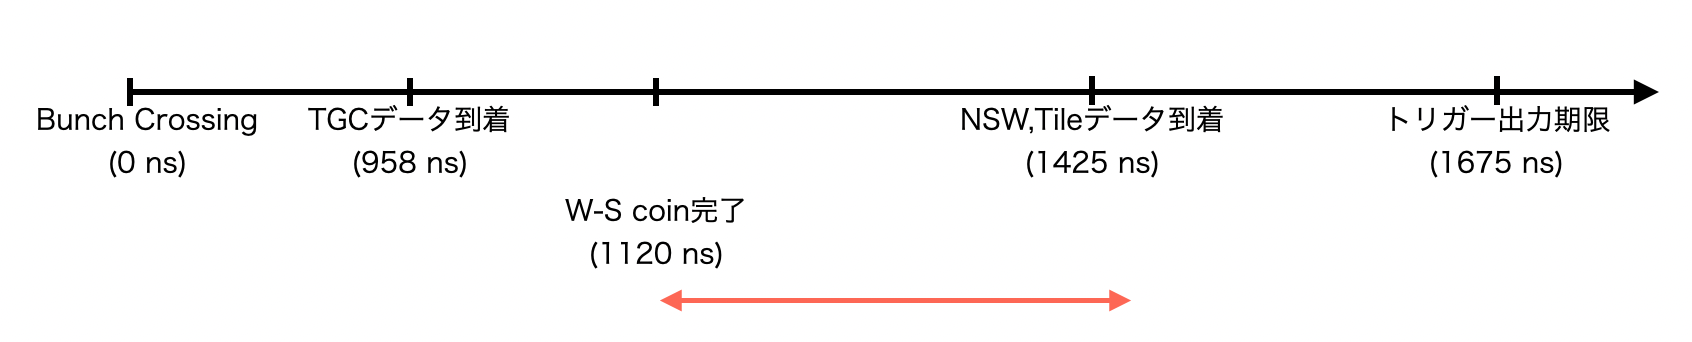
\includegraphics[width=16cm]{fig/SL/Trigger_latency_memo.png}
\caption[トリガーロジックのレイテンシー]{Cトリガーロジックのレイテンシー}
\label{Trigger_latency_memo}
\end{figure}

この2つのことから、Wire Strip Coincidence直後にInner Coincidenceに渡すミューオン候補を絞り込むロジックを挟む最適化を行うことで、トリガー性能を維持したまま、タイミング制約を大幅に緩和できると考えられる。仮にWire Strip Coincidenceから出力されるミューオン候補数を74 個から10個に絞りこんだとすると、SLRをまたぐ信号線は約85 \%程度削減することができる。またInner Coincidenceに並列に実装するロジックの数もこれに合わせて削減することができる。さらに、これに付随してInner Coincidenceから出力されるミューオン候補も自動的に削減されるため、Track Selectorの規模縮小にもつながる。

今後、Inner Coincidenceまでにミューオン候補をどれだけ削減するか、や何を基準に選択するか、などの詳細を決定するためのシミュレーション研究を専攻して進めていく予定である。